%Copyright 2014 Jean-Philippe Eisenbarth
%This program is free software: you can 
%redistribute it and/or modify it under the terms of the GNU General Public 
%License as published by the Free Software Foundation, either version 3 of the 
%License, or (at your option) any later version.
%This program is distributed in the hope that it will be useful,but WITHOUT ANY 
%WARRANTY; without even the implied warranty of MERCHANTABILITY or FITNESS FOR A 
%PARTICULAR PURPOSE. See the GNU General Public License for more details.
%You should have received a copy of the GNU General Public License along with 
%this program.  If not, see <http://www.gnu.org/licenses/>.

%Based on the code of Yiannis Lazarides
%http://tex.stackexchange.com/questions/42602/software-requirements-specification-with-latex
%http://tex.stackexchange.com/users/963/yiannis-lazarides
%Also based on the template of Karl E. Wiegers
%http://www.se.rit.edu/~emad/teaching/slides/srs_template_sep14.pdf
%http://karlwiegers.com
\documentclass{scrreprt}
\usepackage{listings}
\usepackage{underscore}
\usepackage[bookmarks=true]{hyperref}
\usepackage[utf8]{inputenc}
\usepackage[english]{babel}
\usepackage{graphicx}
\hypersetup{
    bookmarks=false,    % show bookmarks bar?
    pdftitle={Software Requirement Specification},    % title
    pdfauthor={Jean-Philippe Eisenbarth},                     % author
    pdfsubject={TeX and LaTeX},                        % subject of the document
    pdfkeywords={TeX, LaTeX, graphics, images}, % list of keywords
    colorlinks=true,       % false: boxed links; true: colored links
    linkcolor=blue,       % color of internal links
    citecolor=black,       % color of links to bibliography
    filecolor=black,        % color of file links
    urlcolor=purple,        % color of external links
    linktoc=page            % only page is linked
}%
\def\myversion{1.0 }
\date{}
%\title
\usepackage{hyperref}
\begin{document}

\begin{flushright}
    \rule{16cm}{5pt}\vskip1cm
    \begin{bfseries}
        \Huge{SOFTWARE REQUIREMENTS\\ SPECIFICATION}\\
        \vspace{1.9cm}
        for\\
        \vspace{1.9cm}
        $<$Project$>$\\
        \vspace{1.9cm}
        \LARGE{Version \myversion approved}\\
        \vspace{1.9cm}
        Prepared by $<$author$>$\\
        \vspace{1.9cm}
        $<$Organization$>$\\
        \vspace{1.9cm}
        \today\\
    \end{bfseries}
\end{flushright}

\tableofcontents


\chapter*{Revision History}

\begin{center}
    \begin{tabular}{|c|c|c|c|}
        \hline
	    Name & Date & Reason For Changes & Version\\
        \hline
	    21 & 22 & 23 & 24\\
        \hline
	    31 & 32 & 33 & 34\\
        \hline
    \end{tabular}
\end{center}

\chapter{Introduction}

\section{Purpose}
This system is designed to interface with SPECjbb 2015 and make it a more user friendly.  The system will provide users with the ability to save an store various run settings for use with SPECjbb 2015. 

\section{Project Scope}
$<$Provide a short description of the software being specified and its purpose, 
including relevant benefits, objectives, and goals. Relate the software to 
corporate goals or business strategies. If a separate vision and scope document 
is available, refer to it rather than duplicating its contents here.$>$

\section{References}
\begin{enumerate}
	\item \hyperlink{https://www.spec.org/jbb2015}{SPECjbb2015}
	\item \hyperlink{https://github.com/PDXCapstoneF/workloads/wiki}{Documentation}
\end{enumerate}


\chapter{Overall Description}

\section{Product Perspective}
This product is a new way to manage configuration files, run SPECjbb 2015, and organize output results. It is specified for benchmark runs on SPECjbb 2015.
\begin{figure}[h!]
	\centering
	\caption[Diagram]{Interface Architecture Diagram}
	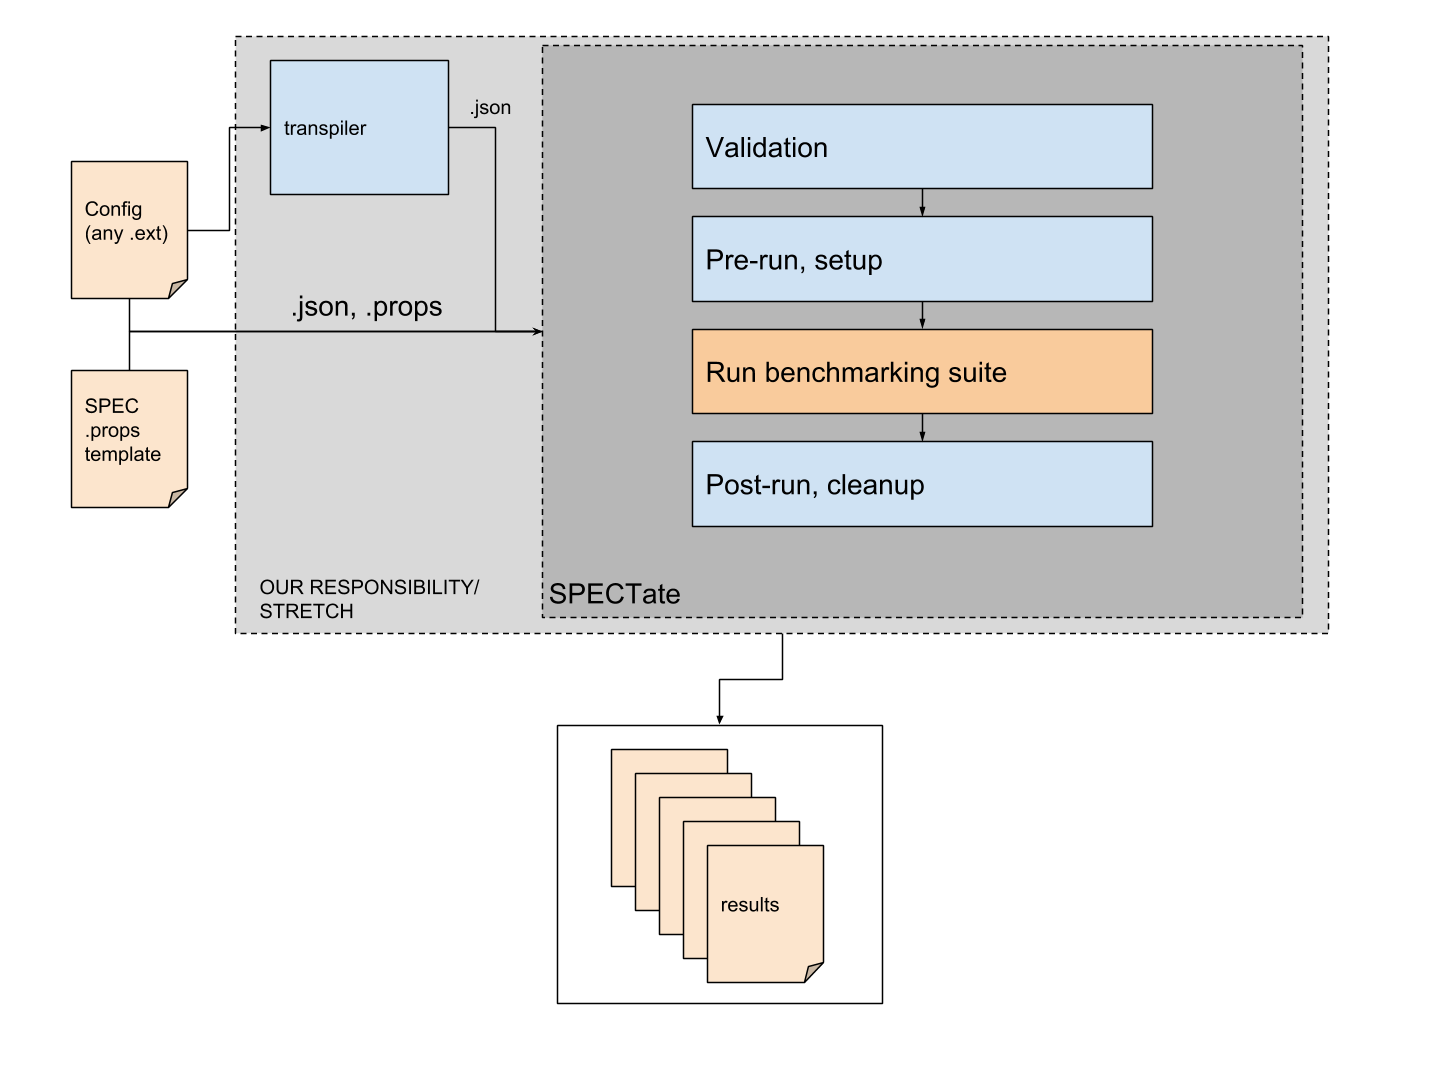
\includegraphics[width=0.8\linewidth]{diagram.png}
	\label{fig:diagram}
\end{figure}

\section{Product Functions}
In general, the product puts focus on a user-friendly way to use SPECjbb 2015, which includes:
\begin{itemize}
	\item Allows queuing multiple SPECjbb jobs to run sequentially with different configuration.
	\item Allows users to create and save a new configuration set or load/modify/delete existed sets.
	\item Allows users to input custom configuration information for SPECjbb.
	\item Provides options/configuration validation.
	\item Provides visualized and organized interface.
\end{itemize}

\section{User Classes and Characteristics}
The product can be found useful to those who are interested in running benchmarks on SPECjbb 2015 in general. More specifically, who are concerned with performance of specific configurations of hardware likely to use SPECjbb more often and the product is necessary. Besides, students and professors from universities or researchers want to consider using SPECjbb in their research is one of important user classes for this product.

\section{Operating Environment}
The application will always run under a Unix environment. Users may run the application remotely without access to a graphical user interface.

\section{Design and Implementation Constraints}
$<$Describe any items or issues that will limit the options available to the 
developers. These might include: corporate or regulatory policies; hardware 
limitations (timing requirements, memory requirements); interfaces to other 
applications; specific technologies, tools, and databases to be used; parallel 
operations; language requirements; communications protocols; security 
considerations; design conventions or programming standards (for example, if the 
customer’s organization will be responsible for maintaining the delivered 
software).$>$

\section{User Documentation}
$<$List the user documentation components (such as user manuals, on-line help, 
and tutorials) that will be delivered along with the software. Identify any 
known user documentation delivery formats or standards.$>$

\section{Assumptions and Dependencies}
$<$List any assumed factors (as opposed to known facts) that could affect the 
requirements stated in the SRS. These could include third-party or commercial 
components that you plan to use, issues around the development or operating 
environment, or constraints. The project could be affected if these assumptions 
are incorrect, are not shared, or change. Also identify any dependencies the 
project has on external factors, such as software components that you intend to 
reuse from another project, unless they are already documented elsewhere (for 
example, in the vision and scope document or the project plan).$>$


\chapter{External Interface Requirements}

\section{User Interfaces}
$<$Describe the logical characteristics of each interface between the software 
product and the users. This may include sample screen images, any GUI standards 
or product family style guides that are to be followed, screen layout 
constraints, standard buttons and functions (e.g., help) that will appear on 
every screen, keyboard shortcuts, error message display standards, and so on.  
Define the software components for which a user interface is needed. Details of 
the user interface design should be documented in a separate user interface 
specification.$>$

\section{Hardware Interfaces}
$<$Describe the logical and physical characteristics of each interface between 
the software product and the hardware components of the system. This may include 
the supported device types, the nature of the data and control interactions 
between the software and the hardware, and communication protocols to be 
used.$>$

\section{Software Interfaces}
$<$Describe the connections between this product and other specific software 
components (name and version), including databases, operating systems, tools, 
libraries, and integrated commercial components. Identify the data items or 
messages coming into the system and going out and describe the purpose of each.  
Describe the services needed and the nature of communications. Refer to 
documents that describe detailed application programming interface protocols.  
Identify data that will be shared across software components. If the data 
sharing mechanism must be implemented in a specific way (for example, use of a 
global data area in a multitasking operating system), specify this as an 
implementation constraint.$>$

\section{Communications Interfaces}
$<$Describe the requirements associated with any communications functions 
required by this product, including e-mail, web browser, network server 
communications protocols, electronic forms, and so on. Define any pertinent 
message formatting. Identify any communication standards that will be used, such 
as FTP or HTTP. Specify any communication security or encryption issues, data 
transfer rates, and synchronization mechanisms.$>$


\chapter{System Features}

\section{System Feature 1}
Option Sets

\subsection{Description and Priority}
Option Sets include all configuration information selected by the user for a single run of SPECjbb 2015.


\subsection{Functional Requirements}
\begin{enumerate}
	\item The system shall allow the user to select any valid JVM on their machine. (\$JAVA)
	\item The system shall validate user provided JVM arguments prior to running SPEC. (\$JAVAOPTS)
	\item The system shall allow the user to select a run type of HBIR, HBIR\_RT, PRESET, or LOADLEVEL\
	\item The system shall allow the user to select the number of runs to be executed.
	\item The system shall allow the user to enable basic data collection. (vmstat -nt 1 $>$ \$RUN\_NUM.vmstat.log \&)
	\item The system shall allow the user to select various SPECjbb options.
	\item The system shall allow the user to input a run identifier (\$TAG)
	\item The system shall allow the user to input the number of Nodes.
\end{enumerate}

\section{System Feature 2}
Option Set execution

\subsection{Description and Priority}
Each Option Set will be executed sequentially.


\subsection{Functional Requirements}
\begin{enumerate}
	\item The system shall inform the user which group and run number is currently executing.
	\item The system shall log all information into SUT.txt
	\item The system shall create a results directory (named \$TAG)
	\item Tge system shall create the configuration file 'specjbb2015.props'
	\item The system shall place the configuration file in the SPEC configuration directory (RC3/config/) prior to running SPEC.
	\item The system shall place a copy of the configuration file in the results directory.
	\item The system shall start the SPEC Controller. (\$JAVA \$JAVAOPTS -jar
	\item The system shall execute each Node appropriately.
	\item The system shall end all started processes once the Controller exits.
	\item The system shall copy all results into the Results Directory (cp result/specjbb2015*/report*/*.html .)
\end{enumerate}
	
	
\section{System Feature 3}
Option Set Node execution

\subsection{Description and Priority}
Users may select each Option Set to be run on a number of different nodes, which must be handled accordingly.


\subsection{Functional Requirements}
	\begin{enumerate}
		\item The system shall inform the user which Node number is being started.
		\item The system shall execute the TxInjector.
		\item The syste m shall execute Backend
	\end{enumerate}
	
	
\section{System Feature 4}
Save, Create, Delete, and Load Option Sets

\subsection{Description and Priority}
The user needs to be create, save, delete, and load Option Sets for quick execution.

\subsection{Functional Requirements}
\begin{enumerate}
	\item Create Option Set
	\item Load Option Set
	\item Delete Option Set
	\item Save Option Set
\end{enumerate}

\section{System Feature 5}
User Interface

\subsection{Description and Priority}
The user needs to be able to visualize and organize Option Sets prior to running benchmarks.

\subsection{Functional Requirements}
\begin{enumerate}
	\item Users need to be able to view available Option Sets
	\item Users need to be able to arrange Option Sets in the order to be executed.
	\item Users need to be able to indicate that they are ready to being benchmarking.
\end{enumerate}

\chapter{Other Nonfunctional Requirements}

\section{Performance Requirements}
$<$If there are performance requirements for the product under various 
circumstances, state them here and explain their rationale, to help the 
developers understand the intent and make suitable design choices. Specify the 
timing relationships for real time systems. Make such requirements as specific 
as possible. You may need to state performance requirements for individual 
functional requirements or features.$>$

\section{Safety Requirements}
$<$Specify those requirements that are concerned with possible loss, damage, or 
harm that could result from the use of the product. Define any safeguards or 
actions that must be taken, as well as actions that must be prevented. Refer to 
any external policies or regulations that state safety issues that affect the 
product’s design or use. Define any safety certifications that must be 
satisfied.$>$

\section{Security Requirements}
$<$Specify any requirements regarding security or privacy issues surrounding use 
of the product or protection of the data used or created by the product. Define 
any user identity authentication requirements. Refer to any external policies or 
regulations containing security issues that affect the product. Define any 
security or privacy certifications that must be satisfied.$>$

\section{Software Quality Attributes}
$<$Specify any additional quality characteristics for the product that will be 
important to either the customers or the developers. Some to consider are: 
adaptability, availability, correctness, flexibility, interoperability, 
maintainability, portability, reliability, reusability, robustness, testability, 
and usability. Write these to be specific, quantitative, and verifiable when 
possible. At the least, clarify the relative preferences for various attributes, 
such as ease of use over ease of learning.$>$

\section{Business Rules}
$<$List any operating principles about the product, such as which individuals or 
roles can perform which functions under specific circumstances. These are not 
functional requirements in themselves, but they may imply certain functional 
requirements to enforce the rules.$>$


\chapter{Other Requirements}
$<$Define any other requirements not covered elsewhere in the SRS. This might 
include database requirements, internationalization requirements, legal 
requirements, reuse objectives for the project, and so on. Add any new sections 
that are pertinent to the project.$>$

\section{Appendix A: Glossary}
%see https://en.wikibooks.org/wiki/LaTeX/Glossary
$<$Define all the terms necessary to properly interpret the SRS, including 
acronyms and abbreviations. You may wish to build a separate glossary that spans 
multiple projects or the entire organization, and just include terms specific to 
a single project in each SRS.$>$

\section{Appendix B: Analysis Models}
$<$Optionally, include any pertinent analysis models, such as data flow 
diagrams, class diagrams, state-transition diagrams, or entity-relationship 
diagrams.$>$

\section{Appendix C: To Be Determined List}
$<$Collect a numbered list of the TBD (to be determined) references that remain 
in the SRS so they can be tracked to closure.$>$

\end{document}